%%
%% This is a LaTeX file template for papers to be
%% submitted to Ecology Letters
%%
%% Companion files required for this template to work properly are:
%% - eco_let.sty, a LaTeX file style to meet the journal's format;
%% - eco_let.bst, a BibTeX file style for the reference list formatting; 
%%
%%

\documentclass[a4paper,12pt,twoside]{article}
\usepackage{ecol_let} %formating style
\usepackage{amssymb} %symbol in equations
\usepackage{amsmath} %equations
\usepackage{rotating}
\usepackage{natbib} %bibliography
\usepackage[flushleft]{threeparttable} %legend and captions in table
\usepackage{float}

\usepackage[draft]{fixme} %annotations
\fxsetup{theme=color,layout=inline}

\usepackage{listings,color} % to insert R code and highlight it
\lstset{
	language=R,
	basicstyle=\footnotesize\ttfamily,
	columns=flexible,
	keepspaces=true,
	% keywordstyle=\color{red},
	% identifierstyle=\color{green},
	commentstyle=\color{blue},
	breaklines=true
}

%numbering instead of lettering for subsections
\renewcommand\thesubsection{\arabic{subsection}}

%fix linenumbers for equations
\newcommand*\patchAmsMathEnvironmentForLineno[1]{%
	\expandafter\let\csname old#1\expandafter\endcsname\csname #1\endcsname
	\expandafter\let\csname oldend#1\expandafter\endcsname\csname end#1\endcsname
	\renewenvironment{#1}%
	{\linenomath\csname old#1\endcsname}%
	{\csname oldend#1\endcsname\endlinenomath}}% 
\newcommand*\patchBothAmsMathEnvironmentsForLineno[1]{%
	\patchAmsMathEnvironmentForLineno{#1}%
	\patchAmsMathEnvironmentForLineno{#1*}}%
\AtBeginDocument{%
	\patchBothAmsMathEnvironmentsForLineno{equation}%
	\patchBothAmsMathEnvironmentsForLineno{align}%
	\patchBothAmsMathEnvironmentsForLineno{flalign}%
	\patchBothAmsMathEnvironmentsForLineno{alignat}%
	\patchBothAmsMathEnvironmentsForLineno{gather}%
	\patchBothAmsMathEnvironmentsForLineno{multline}%
}

\begin{document}
	
	%%%%%%%%%%%%%%%%%%%%%%%%%%%%%%%%%%%%%%%%%%%%%%%%%%%%%%%%%%%%%%%%%%%%%%%%%%%%%%%%%%%%%%
	%%%%%%%%%%%%%% Title page
	%%%%%%%%%%%%%%%%%%%%%%%%%%%%%%%%%%%%%%%%%%%%%%%%%%%%%%%%%%%%%%%%%%%%%%%%%%%%%%%%%%%%%%
	
	%%%%%%%%%%%%%%%%%%%%%%%%%%%%%%%%%%%%%%%%%%%%%%%%%%%%%%%%%%%%%%%%%%%%%%%%%%%%%%%%%%%%%%
	%%%%%%%%%%%%%% Title and running title
	%%%%%%%%%%%%%%%%%%%%%%%%%%%%%%%%%%%%%%%%%%%%%%%%%%%%%%%%%%%%%%%%%%%%%%%%%%%%%%%%%%%%%%
	\shortauthors{Martin et al.}
	\running{Between- and within-individual genetic variance}
	\articletype{Letter}
	\title{Genetic basis of between- and within-individual variance of docility}
	\date{}
	
	%%%%%%%%%%%%%%%%%%%%%%%%%%%%%%%%%%%%%%%%%%%%%%%%%%%%%%%%%%%%%%%%%%%%%%%%%%%%%%%%%%%%%%
	%%%%%%%%%%%%%% List authors and affiliation
	%%%%%%%%%%%%%%%%%%%%%%%%%%%%%%%%%%%%%%%%%%%%%%%%%%%%%%%%%%%%%%%%%%%%%%%%%%%%%%%%%%%%%%
	\author[1]{Julien G.A. Martin\thanks{Corresponding author. Email: julienmartin@abdn.ac.uk, Tel: +44 1224 272399}}
	\author[2]{Enrico Pirotta\thanks{Email: pirotta.enrico@gmail.com}}
	\author[3]{Matthew Petelle\thanks{Email: matthew.petelle@gmail.com}}
	\author[4,5]{Daniel T. Blumstein\thanks{Email: marmots@ucla.edu}}

	\affil[1]{Institute of Biological and Environmental Sciences, University of Aberdeen, Aberdeen, AB24 2TZ, UK}
	\affil[2]{School of Mathematics, Washington State University, 14204 Salmon Creek Avenue, Vancouver WA, 98686, USA}
	\affil[3]{Department of Zoology and Entomology, University of the Free State Qwaqwa, Phuthaditjhaba, South Africa }
	\affil[4]{Department of Ecology and Evolutionary Biology, University of California, Los Angeles, CA, USA}
	\affil[5]{The Rocky Mountain Biological Laboratory, Crested Butte, CO, USA.}
	
	%%%%%%%%%%%%%%%%%%%%%%%%%%%%%%%%%%%%%%%%%%%%%%%%%%%%%%%%%%%%%%%%%%%%%%%%%%%%%%%%%%%%%%
	%%%%%%%%%%%%%% Paper start here
	%%%%%%%%%%%%%%%%%%%%%%%%%%%%%%%%%%%%%%%%%%%%%%%%%%%%%%%%%%%%%%%%%%%%%%%%%%%%%%%%%%%%%%
	\maketitle
	\thispagestyle{empty} 
	
	%%%%%%%%%%%%%%%%%%%%%%%%%%%%%%%%%%%%%%%%%%%%%%%%%%%%%%%%%%%%%%%%%%%%%%%%%%%%%%%%%%%%%%
	%%%%%%%%%%%%%% Keywords
	%%%%%%%%%%%%%%%%%%%%%%%%%%%%%%%%%%%%%%%%%%%%%%%%%%%%%%%%%%%%%%%%%%%%%%%%%%%%%%%%%%%%%%
	\begin{keywords}
		heritability, quantitative genetic, behaviour, personality, dhglm
	\end{keywords}
	
	%%%%%%%%%%%%%%%%%%%%%%%%%%%%%%%%%%%%%%%%%%%%%%%%%%%%%%%%%%%%%%%%%%%%%%%%%%%%%%%%%%%%%%
	%%%%%%%%%%%%%% Author Contribution
	%%%%%%%%%%%%%%%%%%%%%%%%%%%%%%%%%%%%%%%%%%%%%%%%%%%%%%%%%%%%%%%%%%%%%%%%%%%%%%%%%%%%%
	\begin{contribution}
		D.T.B. led the long-term study.
		M.P., D.T.B. and J.G.A.M. collected data.
		J.G.A.M. conceived the ideas for the paper and its structure.
		J.G.A.M. and E.P. designed and conducted the analyses.
		J.G.A.M. wrote the manuscript.
		All authors discussed the results and edited the manuscript. 
	\end{contribution}
	
	\vfill
	%%%%%%%%%%%%%%%%%%%%%%%%%%%%%%%%%%%%%%%%%%%%%%%%%%%%%%%%%%%%%%%%%%%%%%%%%%%%%%%%%%%%%%
	%%%%%%%%%%%%%% Submission info
	%%%%%%%%%%%%%%%%%%%%%%%%%%%%%%%%%%%%%%%%%%%%%%%%%%%%%%%%%%%%%%%%%%%%%%%%%%%%%%%%%%%%%%
	\begin{tabular}{>{\bfseries}lcl}
		Running title &:& Between and within individual genetic variance \\
		Article type &:& Letter\\ 
		Word count &:& 3718 (main text) \\
		Number of references &:& 39 \\
		Number of figures &:& 1 \\
		Number of tables &:& 2 \\
	\end{tabular}
	\vfill
	\newpage
	
	\doublespacing
	%%%%%%%%%%%%%%%%%%%%%%%%%%%%%%%%%%%%%%%%%%%%%%%%%%%%%%%%%%%%%%%%%%%%%%%%%%%%%%%%%%%%%%
	%%%%%%%%%%%%%% Abstract
	%%%%%%%%%%%%%%%%%%%%%%%%%%%%%%%%%%%%%%%%%%%%%%%%%%%%%%%%%%%%%%%%%%%%%%%%%%%%%%%%%%%%%%
	\begin{abstract}
		Within a population, phenotypes vary between and within individuals for labile traits expressed repeatedly.
		However, ecologists have mainly focused on estimating between-individual mean trait variance and neglected variation in predictability (within-individual variance).
		The recent development of double hierarchical models allows concurrent estimation of between-individual differences in both the mean and the predictability of the trait, while correcting for environmental effects. 
		Using long-term data on yellow-bellied marmots, we estimated additive genetic and permanent environment variances in both mean docility and predictability of docility.
		We found that individuals differed not only in their mean docility, but also in their predictability of docility.
		We also found an additive genetic basis and a positive genetic covariance between the mean docility and its predictability. 
		We demonstrate the evolutionary importance of considering variation in predictability of traits, since the additive genetic basis and genetic correlation with the mean trait can influence the evolutionary trajectory of docility.
\end{abstract}
	
	\newpage
	%%%%%%%%%%%%%%%%%%%%%%%%%%%%%%%%%%%%%%%%%%%%%%%%%%%%%%%%%%%%%%%%%%%%%%%%%%%%%%%%%%%%%%
	%%%%%%%%%%%%%% Introduction
	%%%%%%%%%%%%%%%%%%%%%%%%%%%%%%%%%%%%%%%%%%%%%%%%%%%%%%%%%%%%%%%%%%%%%%%%%%%%%%%%%%%%%%
	\section*{Introduction}
	Phenotypic variance is a central concept of ecology and evolution \citep{Roff2002}.
	Phenotypic traits vary among species, among populations, among individuals within populations and, for traits with repeated measures, also within an individual \citep{Roff2002}. 
	Until recently, within-individual variance has been mainly consider to be either due to plasticity and explained by differences in environmental condition \citep{Pigliucci2005, Nussey2007} or due to measurement error \citep{Pigliucci2005, Westneat2014}.
	Studies of between individual variation focused mainly on differences in the mean value of a trait and considered that within individual variance is similar across individuals.
	Indeed, the main assumption of mixed-effects models, a statistical analysis widely used to estimate between-individual variance, is that the residual variance is identical across individuals \citep{Pinheiro2000, Dingemanse2013}. 
	
	In trait repeatedly measured in the same environment, variation in within-individual variance could however be adaptive \citep{Westneat2014, Hill2010}.
	The between individual variation in within-individual variance is being integrated in evolutionary ecology \citep{Mulder2007, Nussey2007} but its study is still at its premise. 
	Studies in animal breeding, using a quantitative genetic approach, have estimated the additive genetic basis of within-genotype variance for multiple productivity related traits such as litter size \citep{Hill2010}, or body weight \citep{Sae-lim2015}.
	The exact evolutionary implications of the genetic basis of within-individual variance and how it affects selection and evolution of the trait is unclear \citep[but see ][]{Mulder2015}.
	The recent development of a framework for its study \citep{Westneat2014, Hill2010} and recent development of statistical methods \cite{Cleasby2015, Mulder2015} should allow for a better understanding of the importance of the variation in within-individual variance.
	
	Currently, one of the biggest problem for the study of within-individual variance differences is lexical. 
	For trait measured repeatedly in the same environmental conditions, multiple terms such as intra-individual variability, individual stability, relative specialisation, consistency, predictability or uniformity are used to refer to variation in within-individual variance \citep{Stamps2012, Cleasby2015, Sae-lim2015}.
	Following, \cite{Cleasby2015}, we are using predictability to refer to within-individual variance in a trait measured repeatedly in the same environment.
	
	The importance and potential impact of variation in predictability of animal behaviour is now widely accepted \citep{Reale2009c, Stamps2012, Westneat2013}.
	However, only a handful of estimates of variation in predictability have been obtained, and often using different non-comparable approaches \citep{Cleasby2015}.
	The recent development of double hierarchical generalized linear model, DHGLM, \citep{Lee2006}, now allows concurrent estimation of between-individual differences in a trait (i.e. variation in the mean) and in its predictability (i.e. variation in within-individual variance) at the same time, while correcting for environmental effects \citep{Cleasby2015}.
	This type of model is an extension of a mixed-effects model fitting fixed and random effects on both the mean and the residual variance of a trait \citep{Lee2006,Cleasby2015}.
	In addition, this approach also allow to obtain comparable parameter of predictability between traits, environments and species \citep{Hill2010, Cleasby2015}.
	
	DHGLM could not only be used to estimate between individual variance in predictability but using a quantitative genetic approach, the variance in predictability could also be decomposed in its additive genetic and environmental effects \citep{Ronnegard2010, Sae-lim2015}.
	To date, only a few estimates of additive genetic variance of predictability of a trait have been published and only in captive animal breeding environment \citep{Mulder2015, Hill2010, Sae-lim2015}.
	Despite its potential importance, existence of genetic basis of predictability in any traits in the wild is unknown.
	Multiple repeated data for a large number of pedigreed individuals is needed to be able to use DHGLM in the wild. 
	In addition,the environment should be measured carefully to ensured that the variation in predictability is not due to uncorrected environmental variation.
	
	
	Variation in predictability of a behaviours is emerging as an important aspect of animal personality \citep{Stamps2012, Cleasby2015, Westneat2014}.
	Animal behaviour, such as docility, could be easy traits to measured repeatedly in standardized conditions in the wild.
	Docility, the reaction to human handling, is a commonly used metric in personality studies, and has been found to be repeatable (ref), heritable (ref), and influence reproduction (ref) in multiple species in the wild. 
	Using long-term trapping data on yellow-bellied, \textit{marmota flaviventris}, we estimated between-individual variation in both mean docility and predictability in docility.
	Using a quantitative genetic approach, we then implemented a “double hierarchical animal model” to decompose the variance of docility and its predictability into their environmental and genetic components.  

	%%%%%%%%%%%%%%%%%%%%%%%%%%%%%%%%%%%%%%%%%%%%%%%%%%%%%%%%%%%%%%%%%%%%%%%%%%%%%%%%%%%%%%
	%%%%%%%%%%%%%% Material and methods
	%%%%%%%%%%%%%%%%%%%%%%%%%%%%%%%%%%%%%%%%%%%%%%%%%%%%S%%%%%%%%%%%%%%%%%%%%%%%%%%%%%%%%%%
	\section*{Material and methods}
	\subsection*{Study system}
	We used behavioural data collected as part of a long-term demographic study on yellow-bellied marmots at the Rocky Mountain Biological Laboratory in Gothic, Colorado, USA (38$^{\circ}$ 77’N, 106$^{\circ}$ 59’W).
	Marmots are large, facultatively social, subalpine rodents that live in colonies consisting of one or more matrilineal groups \citep{Frase1980, Armitage2014}. 
	These colonies usually consist of one adult male, multiple adult females, and their offsprings. 
	We regularly trap individuals using Tomahawk live traps set at burrow entrances. 
	Once trapped, individuals were weighed, sexed, their ano-genital distance and left hind foot measured, ear tagged, and given an unique dye mark to facilitate identification from afar \citep{Blumstein2009}. 
	
	Docility was assessed as an individual’s reaction to being trapped and handled \citep{Reale2007, Petelle2013}.
	Upon arriving at a trap, individuals were placed inside a cloth-handling bag, and we dichotomously scored (0, 1) whether individuals bit the trap, emitted an alarm called, struggled in the trap or bag, tooth chattered, and whether they hesitated moving from the trap into the handling bag. 
	We summed these scores and subtracted them from a maximum of five. 
	Thus, a docile individual would have a score of five while an individual with a score of 0 would be non-docile or pugnacious \citep{Reale2007}. 
	We quantified docility over 11,389 trapping events for 1,576 individuals of known age and sex from 2002-2014. Mean and range of docility observations varied widely across individuals (Fig.~\ref{Fig:rawdata}).
	
	Parentage was assigned from DNA samples collected from individuals during their first trapping event.
	We extracted DNA using a QiaGen QIAamp DNA minikit and genotyped individuals using 12 microsatellites. 
	Alleles were visualized and assigned using GeneMapper 4.1 software (Applied Biosystems). 
	CERVUS \citep{Kalinowski2007} was then used to assign maternity and paternity using a maximum likelihood method at 95\% confidence for the trio. All adult males and females in a colony were used as potential parents.
	Genetic assignments of maternity confirmed behavioural observations based on juveniles emergence from maternal burrow.
	For full details on the pedigree reconstruction method see \cite{Olson2012} and \cite{Blumstein2010}.
	The pedigree used in these analyses included 1588 individuals with 90\% and 83\% of the maternal and paternal links known respectively (see Table~\ref{Tab:pedigree} for detailed pedigree structure information).
	
	\subsection*{Statistical analysis}
	The aim of our analysis was to concurrently estimate the between-individual differences in mean docility and its predictability (residual within-individual variance). 
	Moreover, we wanted to decompose the variability of the mean trait and of its predictability into environmental and genetic components using a quantitative genetic approach. 
	We developed four models differing in their random and residual structure that progressively built towards such goal, while allowing us to monitor any change in the estimates as increasing complexity was introduced (see Table~\ref{Tab:models}). 
	Following previous results from this population \citep{Petelle2013, Petelle2015}, we included the following fixed effects in the mean part of all models: trial number, to account for potential habituation to human handling; day of the year, as a proxy for any seasonal changes in docility; time of day, coded as 0 for AM sampling and 1 for PM sampling; and age, which was a categorical factor with three levels (juveniles, yearlings and adults).
	
	Model 1 was a traditional mixed-effects model, where the mean docility was modelled as a combination of fixed and random effects and variance was assumed to be homogeneous across individuals. 
	Model 1 can be therefore written as:
	\begin{equation}\label{Eq:mm}
	\boldsymbol{Y} = \boldsymbol{X_m b_m} + \boldsymbol{M yr_m} + \boldsymbol{Z pe_m} + \boldsymbol{e}
	\end{equation}
	where $\boldsymbol{yr_m} \sim N(0, \boldsymbol{I}\sigma_{yr_m}^2)$, $\boldsymbol{pe_m} \sim N(0, \boldsymbol{I}\sigma_{pe_m}^2)$ and $\boldsymbol{e} \sim N(0, \boldsymbol{I}\sigma_e^2)$).
	$\boldsymbol{Y}$ is the vector of docility records. 
	$\boldsymbol{b_m}$, $\boldsymbol{yr_m}$ and $\boldsymbol{pe_m}$ are the vectors of fixed, random year and permanent environmental (identity) effects associated with the corresponding incidence matrix $\boldsymbol{X_m}$, $\boldsymbol{M}$ and $\boldsymbol{Z}$. 
	$\boldsymbol{e}$ is the vector of residuals with variance $\sigma_e^2$. 
	$\sigma_{yr_m}^2$ and $\sigma_{pe_m}^2$ are the between-year and between-individual random effect variances, respectively. 
	$\boldsymbol{I}$ is the identity matrix. 
	
	Similarly to model 1, model 2 only considered changes in mean docility. 
	However, this model also included an additive genetic component, fitted as a random effect on the mean \citep{Waldmann2009}.
	Model 2 is therefore equivalent to a classic animal model \citep{Kruuk2004}, and can be written as:
	\begin{equation}\label{Eq:am}
	\boldsymbol{Y} = \boldsymbol{X_m b_m} + \boldsymbol{M yr_m} + \boldsymbol{Z pe_m} + \boldsymbol{Z a_m} + \boldsymbol{e}
	\end{equation}
	where, building on equation~\ref{Eq:mm}, $\boldsymbol{a_m} \sim N(0, \boldsymbol{A}\sigma_{a_{m}}^2)$.
	$\boldsymbol{a_m}$ is the vector of additive genetic effects. 
	Since each individual has an additive genetic as well as a permanent environmental effect, both effects have the same design matrix $\boldsymbol{Z}$.
	$\sigma_{a_{m}}^2$ is the additive genetic variance of the mean trait and $\boldsymbol{A}$ is the additive genetic relationship matrix.
	
	Model 3 was a double hierarchical generalised linear model (DHGLM) \citep{Lee2006,Cleasby2015}.
	This included a model for the mean docility (as in model 1), as well as a dispersion part for the residual variance ()i.e. predictability).
	Following \cite{Sancristobal-gaudy1998}, the residual variance was modelled on the log-normal scale as a function of the fixed effect of age, with year and individual identity as random effects.
	We also estimated the correlation between the individual random effect on the mean and on the within-individual variance, using a multivariate Normal distribution.
	Model 3 can be written as:
	\begin{equation}\label{Eq:dhm}
		\begin{aligned}
			&\boldsymbol{Y} = \boldsymbol{X_m b_m} + \boldsymbol{M yr_m} + \boldsymbol{Z pe_m} + \boldsymbol{e}\\
			&\log (\boldsymbol{\sigma_e^2}) = \boldsymbol{X_v b_v} + \boldsymbol{M yr_v} + \boldsymbol{Z pe_v}
		\end{aligned}
	\end{equation}
	where $\boldsymbol{e} \sim N \left(0, Diag [ \boldsymbol{\sigma_e^2}] \right) $, $\boldsymbol{yr_v} \sim N \left( 0, \boldsymbol{I}\sigma_{yr_{v,exp}}^2 \right) $, 
	$\begin{bmatrix}
		\boldsymbol{pe_m} \\
		\boldsymbol{pe_v}
	\end{bmatrix}
	\sim N \left(\begin{matrix} 0 \\ 0 \end{matrix}, \Sigma_{pe} \otimes \boldsymbol{I} \right)$
	and
	$\Sigma_{pe} =
	\begin{bmatrix}
		\sigma_{pe_m}^2 & \sigma_{pe_m}\sigma_{pe_{v,exp}}\rho_{pe} \\
		\sigma_{pe_m}\sigma_{pe_{v,exp}}\rho_{pe} & \sigma_{pe_{v,exp}}^2 
	\end{bmatrix}
	$.
	Building on equation~\ref{Eq:mm}, $\boldsymbol{\sigma_e^2}$ is now a vector and $Diag()$ is used to create a diagonal matrix.
	$\boldsymbol{b_v}$, $\boldsymbol{yr_v}$ and $\boldsymbol{pe_v}$ are the vectors of fixed, random year and random permanent environmental (identity) effects associated with the corresponding incidence matrix $\boldsymbol{X_v}$, $\boldsymbol{M}$ and $\boldsymbol{Z}$.
	$\sigma_{yr_{v,exp}}^2$ and $\sigma_{pe_{v,exp}}^2$ are the year and permanent environmental variance of the within-individual variance on the exponential scale.
	$\rho_{pe}$ is the correlation at the individual level between the mean trait and the within-individual variance of the trait.
	
	Finally, model 4 was a double hierarchical generalised linear "animal" model (DHGLAM), with a mean and a dispersion part as in model 3, but including an additive genetic component (as in model 2) fitted as a correlated random effect on both the mean and the within-individual variance \citep{Felleki2012}.
	Starting from Equation~\ref{Eq:dhm}, model 4 can therefore be written as:
	\begin{equation}\label{Eq:dham}
		\begin{aligned}
			&\boldsymbol{Y} = \boldsymbol{X_m b_m} + \boldsymbol{M yr_m} + \boldsymbol{Z pe_m} + \boldsymbol{Z a_m} + \boldsymbol{e}\\
			&\log (\boldsymbol{\sigma_e^2}) = \boldsymbol{X_v b_v} + \boldsymbol{M yr_v} + \boldsymbol{Z pe_v} + \boldsymbol{Z a_v}
		\end{aligned}
	\end{equation}
	where 
	$\begin{bmatrix}
		\boldsymbol{a_m} \\
		\boldsymbol{a_v}
	\end{bmatrix}
	\sim N \left(\begin{matrix} 0 \\ 0 \end{matrix}, \Sigma_a \otimes \boldsymbol{A} \right)
	$
	and $\Sigma_a =
	\begin{bmatrix}
		\sigma_{a_m}^2 & \sigma_{a_m}\sigma_{a_{v,exp}}\rho_{a} \\
		\sigma_{a_m}\sigma_{a_{v,exp}}\rho_{a} & \sigma_{a_{v,exp}}^2 
	\end{bmatrix}$.
	$\boldsymbol{a_v}$ is the vectors of additive genetic effects associated with the corresponding incidence matrix $\boldsymbol{Z}$. 
	$\sigma_{a_{v,exp}}^2$ is the additive genetic variance of the within-individual variance on the exponential scale and $\rho_{a}$ is the additive genetic correlation between the mean and within-individual variance.
	
	The estimated variance components ($\sigma_{yr_{v,exp}}^2$, $\sigma_{pe_{v,exp}}^2$ and $\sigma_{a_{v,exp}}^2$) for the predictability of docility were on the exponential scale (exp) and were converted to an additive scale ($\sigma_{yr_v}^2$, $\sigma_{pe_v}^2$ and $\sigma_{a_v}^2$) using the equations derived by \cite{Mulder2007} (see also Appendix~\ref{ESM:equations}).
	For each model, we estimated the phenotypic variance conditioned on the fixed effects ($\sigma_P^2$) as the sum of the variance components and the residual variance ($\sigma_e^2$).
	For model 3 and 4, $\sigma_e^2$ was estimated as $\exp \left( b_{v_0} + \frac{b_{v_1}}{3}+ \frac{b_{v_2}}{3} \right) \exp \left( \frac{\sigma_{yr_{v,exp}}^2}{2} \right) \exp \left( \frac{\sigma_{pe_{v,exp}}^2}{2} \right) \exp \left( \frac{\sigma_{a_{v,exp}}^2}{2} \right)$ \citep[Appendix~\ref{ESM:equations};][]{Felleki2012, Sae-lim2015}.
	For all models, repeatability (or permanent environment effect, $pe^2$) for mean docility was estimated as $\frac{\sigma_{pe_m}^2}{ \sigma_P^2 }$ and for within-individual variance in docility ($pe_v^2$) as $\frac{\sigma_{pe_v}^2}{2\sigma_P^4+3(\sigma_{yr_v}^2+ \sigma_{pe_v}^2 + \sigma_{a_v}^2)}$.
	Similarly heritability of docility ($h^2$) and of within-individual variance in docility ($h_v^2$) were estimated as $\frac{\sigma_{a_m}^2}{ \sigma_P^2 }$ and $\frac{\sigma_{a_v}^2}{2\sigma_P^4+3(\sigma_{yr_v}^2+ \sigma_{pe_v}^2 + \sigma_{a_v}^2)}$, respectively \citep[Appendix~\ref{ESM:equations};][]{Mulder2007}.
	We also reported the permanent environment and genetic coefficient of variation of the within-individual variance on the additive scale estimated as $CV_{{pe}_v} = \frac{\sigma_{{pe}_v}}{\sigma_e^2}$ and $CV_{a_v} = \frac{\sigma_{a_v}}{\sigma_e^2}$ respectively \citep{Hill2010}.

	
	
	The four models were fitted in a Bayesian framework using OpenBUGS 3.2.1 \citep{Thomas2006}, run from R \citep{RDevelopmentCoreTeam2014} via the package R2OpenBUGS \cite{Sturtz2005}. Quantitative genetic effects were implemented in BUGS following \cite{Waldmann2009} and \cite{Gorjanc2010}.
	We used Normal priors with mean 0 and precision 0.001 for the fixed effects in both the mean and dispersion part.
	$\sigma_e$ had a uniform prior $U(0,20)$, and $\sigma_{yr_m}$ and $\sigma_{yr_v}$ had uniform priors $U(0,10)$.
	In model 1 and 2, $\sigma_{pe_m}$ had a uniform prior $U(0,10)$, while in model 3 and 4, $\Sigma_{pe}$ had an inverse Wishart prior with 3 degrees of freedom and scale matrix $\begin{bmatrix} 1 & 0 \\ 0 & 1 \end{bmatrix}$.
	In model 2, $\sigma_{a_m}$ had a uniform prior $U(0,15)$, while for $\Sigma_{a}$ in model 4, we used an inverse Wishart prior with 3 degrees of freedom and scale matrix $\begin{bmatrix} 1 & 0 \\ 0 & 1 \end{bmatrix}$.
	The OpenBUGS code for model 4 is provided in the Supplementary material (ESM~\ref{ESM:bugscode}).
	Markov Chain Monte Carlo (MCMC) algorithms were iterated until convergence to the joint posterior distribution.
	Three chains starting at different initial values were run in parallel.
	Convergence was first assessed by visually inspecting the trace plots, which were also used to identify an appropriate number of burn-in iterations. 
	Each chain ran for 270,000 iterations including 70,000 burn-in iterations.
	We then checked that the Monte Carlo error was less than 1-5\% of the posterior standard deviation, and that the Brooks-Gelman-Rubin (BGR) diagnostic converged to 1 $\pm$ 0.2 \cite{Gilks1995}.
	These convergence checks were carried out using the package coda \citep{Plummer2006} in R.
	The mode and 95\% Highest Posterior Density Intervals (HPDI) were used to summarise the posterior distributions of the model parameters. 
	Results are reported using the combined 600,000 iterations from the 3 unthinned chains following \citep{Link2012,Kruschke2014}.
	
	%%%%%%%%%%%%%%%%%%%%%%%%%%%%%%%%%%%%%%%%%%%%%%%%%%%%%%%%%%%%%%%%%%%%%%%%%%%%%%%%%%%%%%
	%%%%%%%%%%%%%% Results
	%%%%%%%%%%%%%%%%%%%%%%%%%%%%%%%%%%%%%%%%%%%%%%%%%%%%%%%%%%%%%%%%%%%%%%%%%%%%%%%%%%%%%%
	\section*{Results}
	We found that parameter estimates for both fixed and random effects across all models were highly consistent (Fig.~\ref{Fig:yr}), Table~\ref{Tab:estimates}) validating the approach used.
	Trial number and age had a significant effect on the mean part of all models (estimated as 95\% HDPI not overlapping zero). Age was also significant in the dispersion part of both model 3 and 4 (Fig.~\ref{Fig:yr}).
	However, time of the day had no significant effect when also modelling the dispersion of docility (model 3 and 4, Fig.~\ref{Fig:yr}).
	
	As previously reported \citep{Petelle2015}, we found significant repeatability ($pe^2$) and heritability ($h^2$) of docility (Table~\ref{Tab:estimates}) with similar estimates when comparing hierarchical models (models 1, 2) with double hierarchical models (models 3, 4).
	More importantly, we found significant permanent environment and additive genetic variance in the predictability of docility (Fig.~\ref{Fig:yr}, Table~\ref{Tab:estimates}) with estimated repeatability ($pe_v^2$) and heritability ($h_v^2$) equal to 0.09 (95\%HPDI: 0.07/0.11) and 0.07 (0.05/0.10) respectively.
	In addition, both permanent environment and additive genetic correlation between the mean and the within-individual variance were negative and significantly different from zero (Fig.~\ref{Fig:yr}, Table~\ref{Tab:estimates}).
	
	Permanent environment variance ($\sigma_{pe}^2$) for the mean is consistent across model 1 and 3, and across model 2 and 4 (Fig.~\ref{Fig:yr}, Table~\ref{Tab:estimates}).
	The difference in ($\sigma_{pe}^2$) between models 1, 3 and models 2, 4 results from the addition of the additive genetic effect in models 2 and 4.
	In models 2 and 4, the sum of the additive genetic ($\sigma_{a}^2$) and permanent environmental ($\sigma_{pe}^2$) variances are consistent with the estimates of ($\sigma_{pe}^2$) in model 1 and 3 indicating that the models are behaving adequately (Table~\ref{Tab:estimates}).
	As with the mean part of the model, the sum of the additive genetic ($\sigma_{a_v}^2$) and permanent environmental ($\sigma_{pe_v}^2$) variances in the dispersion part of model 4 are consistent with the estimates of ($\sigma_{pe_v}^2$) in model 3 (Table~\ref{Tab:estimates}).
	
	The random effect of year was negligible in both the mean and the dispersion part of the models (Fig.~\ref{Fig:yr}, Table~\ref{Tab:estimates}).
	We then refitted the models without year as a random effect in either the mean or the dispersion part of the model Table~\ref{Tab:modelsnoyr} and found both qualitatively and quantitatively similar results (Fig.~\ref{Fig:noyr} and Table~\ref{Tab:estimatesnoyr}).
	
	%%%%%%%%%%%%%%%%%%%%%%%%%%%%%%%%%%%%%%%%%%%%%%%%%%%%%%%%%%%%%%%%%%%%%%%%%%%%%%%%%%%%%%
	%%%%%%%%%%%%%% Discussion (section 4)
	%%%%%%%%%%%%%%%%%%%%%%%%%%%%%%%%%%%%%%%%%%%%%%%%%%%%%%%%%%%%%%%%%%%%%%%%%%%%%%%%%%%%%%
	\section*{Discussion}
	The long-term data available for the RMBL yellow-bellied marmot provide a valuable opportunity to develop our understanding of between individual differences in within-individual variation.
	We found three major results with strong implications for our understanding of behaviour evolution.
	First, we found that contrary to most studies on behaviours that homogeneous within-individual variance across individuals should not be assumed.
	Second, we showed a significant additive genetic variance in predictability (i.e. within-individual variance) of docility.
	Third, we found a significant negative genetic correlation between mean docility and its predictability.
	These analyses are, to our knowledge, the first to estimate the genetic basis of both mean trait and its predictability in a wild population for any trait not only a behavioural trait. 
		
	Our results are quantitatively similar to previous estimates of heritability for predictability of life-history trait, $h_v^2$, and their coefficient of genetic variation $CV_{a_v}$ obtained on captive animal \citep{Hill2010}.
	The estimate of $h_v^2$ is low in part because predictability of docility can be affected by multiple environmental factors that reduce heritability \citep{Houle1992, Westneat2014}.
	Also we found low estimate of heritability for predictability of docility, its coefficient of genetic variation was high 42.1\% which indicates a high potential for genetic change in response to selection for higher predictability relative to the mean \citep{Mulder2007, Hill2010}.
	The existence of $h_v^2$ for docility might indicated that the variation in the within-individual variance is adaptive \citep{Westneat2014}.
	The mechanisms underlying such variance are not clear and might include phenotype switching, polyphenisms and diversification bet-hedging \citep{Westneat2014}.
	However, importance of the predictability of a trait for survival or reproduction has not been studied yet.

	Predictability of docility could not only be under selection and evolve but selection on predictability of docility will indirectly impact evolution of docility because of the negative genetic correlation between docility and its predictability.
	Inversely, selection on mean docility will indirectly affect the predictability of docility.	
	The evolutionary implications of the existence of additive genetic basis for the predictability of a trait are not clear yet \citep{Mulder2015}.
	Correlations between the predictability of a trait and the mean level of another trait is expected to lead to nonlinearity between the two traits \citep{Mulder2015}.
	However, the impact of direct selection on the predictability of a trait or the impact existence of genetic correlation between predictability of two different traits on the evolution of mean traits have not been investigated so far.
	It is fair to say that the implications of additive genetic basis for the predictability of a trait under multivariate selection on both mean traits and their predictability is not fully understood.
	As indicated by \cite{Westneat2014}, this should be a promising area of research in the future.

	In this study, we also show a framework to estimate predictability of a trait and to calculate estimates comparable across populations, traits and studies ((ESM~\ref{ESM:equations})).
	Based on work by \cite{Mulder2007} and \cite{Sae-lim2015}, we presented the equations to estimate repeatability $r_v^2$ and heritability $h_v^2$ of  the predictability of a trait when multiple random effects are fitted in the dispersion part of the model. 
	The method presented in \cite{Cleasby2015} allows only to fit individual identity as a random effect in the dispersion part of the model to estimate the index of predictability.
	It should be noted that the equation in \cite{Cleasby2015} for the coefficient of variation estimated on the exponential scale is valid only with 1 random effect for the within-individual variance (i.e. dispersion part of the model) and thus not appropriate in our situation.
	For these equations, it is assumed that the genetic ($r_a$) and permanent environmental ($r_{pe}$) correlations between mean and predictability variance are 0 \citep{Mulder2007}.
	Even if the effect of this simplifying assumption seems to be weak \citep{Mulder2007, Sae-lim2015}, $h_v^2$ should be used only as a first approximation in standard prediction evolutionary model when the genetic correlation differs from 0 (see \cite{Mulder2007} for complete equations).
		
	To our knowledge this is the only study to have estimated the genetic variance and covariance between a trait and its predictability (i.e. within-individual variance) in a wild-living animal population.
	We also illustrate that heritability and other variance ratio could be estimated using double hierarchical animal models and argued that they should be used over other estimates for easier comparison between population, species and studies \citep{Stamps2012,Cleasby2015,Reale2009c}.
	
	%%%%%%%%%%%%%%%%%%%%%%%%%%%%%%%%%%%%%%%%%%%%%%%%%%%%%%%%%%%%%%%%%%%%%%%%%%%%%%%%%%%%%%
	%%%%%%%%%%%%%% Acknowledgments
	%%%%%%%%%%%%%%%%%%%%%%%%%%%%%%%%%%%%%%%%%%%%%%%%%%%%%%%%%%%%%%%%%%%%%%%%%%%%%%%%%%%%%%
	\section*{Acknowledgments}
	%\begin{small}
	We thank all the ‘marmoteers’ who participated in collecting the long-term data, and the Rocky Mountain Biological Laboratory for providing the field facilities. 
	This work was funded by the UCLA Academic Senate and Division of Life Sciences, National Geographic Society, and NSF-IDBR-0754247, NSF- DEB-1119660 (to D.T.B.); NSF-DBI 0242960, 0731346 (to the RMBL), and by the Univeristy of Aberdeen and Marie-Curie Actions (to J.M.).
	%\end{small}
	
	%%%%%%%%%%%%%%%%%%%%%%%%%%%%%%%%%%%%%%%%%%%%%%%%%%%%%%%%%%%%%%%%%%%%%%%%%%%%%%%%%%%%%%
	%%%%%%%%%%%%%% References
	%%%%%%%%%%%%%%%%%%%%%%%%%%%%%%%%%%%%%%%%%%%%%%%%%%%%%%%%%%%%%%%%%%%%%%%%%%%%%%%%%%%%%%
	\bibliography{dhglmDocility}

	
	
	%%%%%%%%%%%%%%%%%%%%%%%%%%%%%%%%%%%%%%%%%%%%%%%%%%%%%%%%%%%%%%%%%%%%%%%%%%%%%%%%%%%%%%
	%%%%%%%%%%%%%% Tables
	%%%%%%%%%%%%%%%%%%%%%%%%%%%%%%%%%%%%%%%%%%%%%%%%%%%%%%%%%%%%%%%%%%%%%%%%%%%%%%%%%%%%%% 
	\newpage
	\section*{Tables}
	
	\begin{table}[!ht]
		\caption{Fixed and random effects fitted in each model of docility in yellow-bellied marmots at RMBL. 
			ID represents a permanent environmental effects whereas AG represents additive genetic effects.}
		\label{Tab:models}
		\centering
		\begin{tabular}{c c c c c}
			\hline
			\multicolumn{1}{c}{} &
			\multicolumn{2}{c}{Mean part effects} &
			\multicolumn{2}{c}{Dispersion part effects}\\ 
			Model & Fixed & Random & Fixed & Random \\
			\hline
			1 & Trial + Date + Time + Age & Year + ID & & \\
			2 & Trial + Date + Time + Age & Year +ID + AG & & \\
			3 & Trial + Date + Time + Age & Year + ID & Age & Year + ID \\
			4 & Trial + Date + Time + Age & Year + ID + AG & Age & Year + ID + AG\\
			\hline
		\end{tabular}
	\end{table}
	\newpage
	
	
	\begin{table}[ht!]
		\caption{Estimates of variance components and variance ratios of docility for the four different models differing in their random and residual structure (see table 1). 
			Analysis used 11,389 observations from 1,576 individuals between 2002-2014.}
		\label{Tab:estimates}
		\centering
		\small
		\begin{tabular}{c c c c c}
			\hline
			\multicolumn{1}{c}{} &
			\multicolumn{4}{c}{Models}\\
			& 1 & 2 & 3 & 4\\
			\hline
			$\sigma_P^2$ & 0.872 (0.903/0.999) & 0.959 (0.918/1.004) & 0.995 (0.892/1.126) & 1.251 (1.075/1.494)\\
			Mean part & & & &\\
			$\sigma_{yr}^{2}$ & 0.003 (0.005/0.059) & 0.012 (0.004/0.038) & 0.012 (0.005/0.038) & 0.01 (0.004/0.031)\\
			$\sigma_{pe}^2$ & 0.215 (0.185/0.243) & 0.099 (0.073/0.129) & 0.18 (0.16/0.205) & 0.105 (0.083/0.128)\\
			$\sigma_{a}^2$ & - & 0.132 (0.09/0.18) & - & 0.097 (0.069/0.132)\\
			$year^2$ & 0.016 (0.006/0.061) & 0.013 (0.005/0.039) & 0.012 (0.005/0.037) & 0.008 (0.003/0.024)\\
			$pe^2$ & 0.227 (0.196/0.256) & 0.102 (0.075/0.135) & 0.183 (0.156/0.208) & 0.081 (0.059/0.107)\\
			$h^2$ & - & 0.14 (0.096/0.183) & - & 0.078 (0.055/0.103)\\
			Dispersion part & & & &\\
			$\sigma_{yr_{v, exp}}^2$ & - & - & 0.03 (0.011/0.092) & 0.026 (0.01/0.086)\\
			$\sigma_{pe_{v, exp}}^2$ & - & - & 0.657 (0.577/0.749) & 0.391 (0.304/0.484)\\
			$\sigma_{a_{v, exp}}^2$ & - & - & - & 0.289 (0.189/0.418)\\
			$year_v^2$ & - & - & 0.007 (0.003/0.021) & 0.007 (0.002/0.02)\\
			$pe_v^2$ & - & - & 0.154 (0.139/0.171) & 0.093 (0.073/0.115)\\
			$h_v^2$ & - & - & - & 0.069 (0.046/0.098)\\
			$CV_{year_v}$ & - & - & 0.030 (0.011/0.114) & 0.040 (0.013/0.141)\\
			$CV_{pe_v}$ & - & - & 0.730 (0.584/0.984) & 0.587 (0.425/0.818)\\
			$CV_{a_v}$ & - & - & - & 0.421 (0.243/0.737)\\
			Covariance & & & &\\
			$cov_{pe}$ & - & - & -0.324 (-0.364/-0.293) & -0.183 (-0.225/-0.144)\\
			$cov_{a}$ & - & - & - & -0.149 (-0.208/-0.096)\\
			$cor_{pe}$ & - & - & -0.944 (-0.958/-0.929) & -0.907 (-0.931/-0.871)\\
			$cor_{a}$ & - & - & - & -0.876 (-0.919/-0.811)\\
			\hline
		\end{tabular}
		\begin{tablenotes}
			\small
			\item $\sigma_P^2$ = estimated phenotypic variance.
			$\sigma_a^2$ and $\sigma_{a_{v, exp}}^2$ = additive genetic variance for mean docility and predictability docility on the exponential scale, respectively. 
			$\sigma_{pe}^2$= permanent environmental variance, $\sigma_{yr}^2$ = year variance. 
			$h^2$ and $h_v^2$ = heritability for mean docility and predictability of docility, respectively. 
			$pe^2$ = permanent environmental (2 and 4) or repeatability (1 and 3) estimates. 
			$year^2$ = year effect.
			$CV_{year_v}$, $CV_{pe_v}$ and $CV_{a_v}$ are the coefficient of variance for the random effects fitted on predictability of docility.
		\end{tablenotes}
	\end{table}
	
	
	
	
	%%%%%%%%%%%%%%%%%%%%%%%%%%%%%%%%%%%%%%%%%%%%%%%%%%%%%%%%%%%%%%%%%%%%%%%%%%%%%%%%%%%%%%
	%%%%%%%%%%%%%% Figures
	%%%%%%%%%%%%%%%%%%%%%%%%%%%%%%%%%%%%%%%%%%%%%%%%%%%%%%%%%%%%%%%%%%%%%%%%%%%%%%%%%%%%%%
	\newpage
	\section*{Figures}
	\begin{figure}[ht!]
		\caption{Posterior mode and 95\% credible intervals for four different models of docility of Yellow-bellied marmots at RMBL. 
			Analysis used 11,389 observations from 1,576 individuals over between 2002-2014. 
			Grey shaded area illustrates an invalid region of the parameter space. 
			Residual variance ($\sigma_e^2$) for models 3 and 4 were estimated based on Appendix \ref{ESM:equations}. 
			Juvenile was considered as references in both mean and variance part of the model.
			3.7 was subtracted from the estimates of the intercept to facilitate plotting}
		\label{Fig:yr}
		\begin{center}
			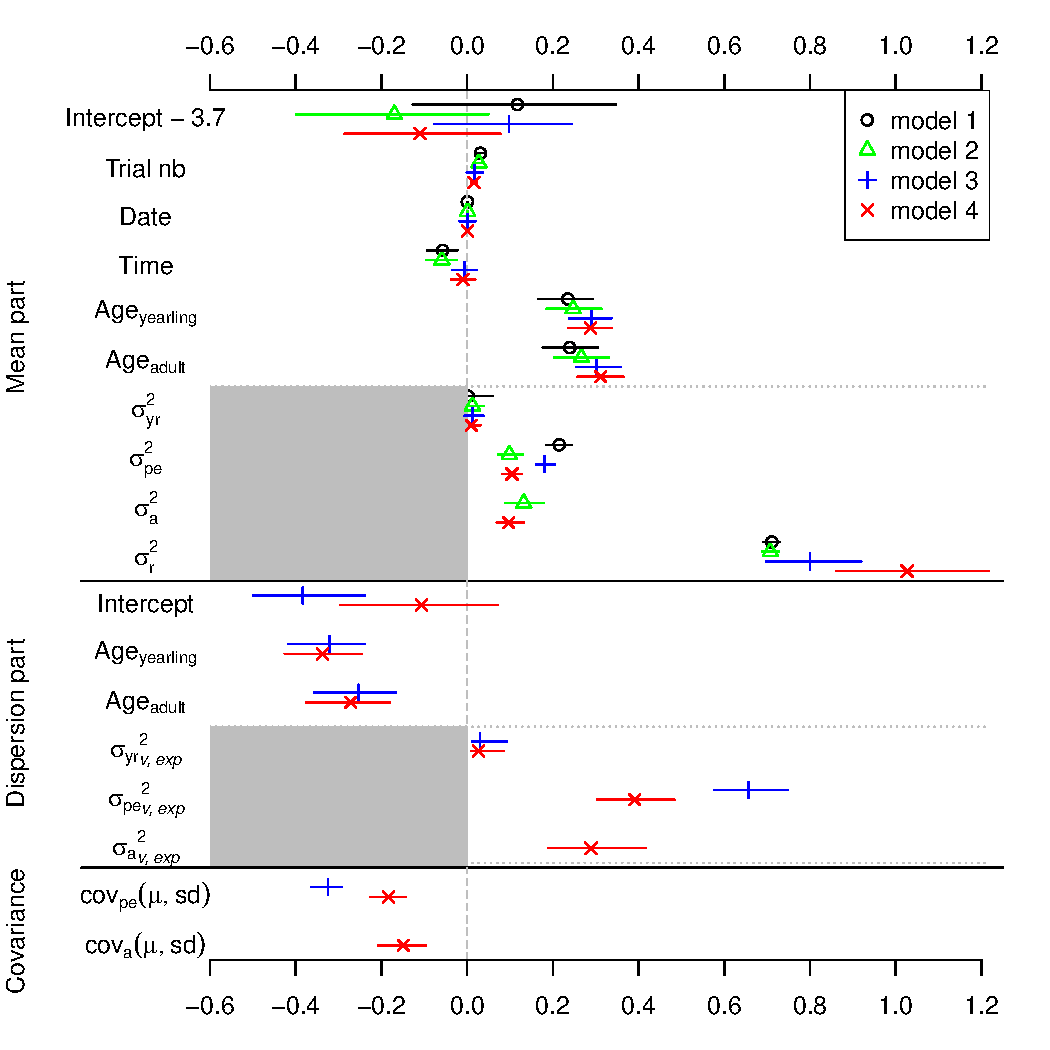
\includegraphics[width=14cm]{Fig1year.pdf}
		\end{center}
	\end{figure}
	
	
	%%%%%%%%%%%%%%%%%%%%%%%%%%%%%%%%%%%%%%%%%%%%%%%%%%%%%%%%%%%%%%%%%%%%%%%%%%%%%%%%%%%%%%
	%%%%%%%%%%%%%% appendix
	%%%%%%%%%%%%%%%%%%%%%%%%%%%%%%%%%%%%%%%%%%%%%%%%%%%%%%%%%%%%%%%%%%%%%%%%%%%%%%%%%%%%%%
	\newpage
	\section*{Electronic Supplementary Materials}
	\setcounter{table}{0}
	\setcounter{figure}{0}
	\renewcommand{\thetable}{S\arabic{table}}
	\renewcommand{\thefigure}{S\arabic{figure}}
	
	
	\noindent Appendix S1. Supplementary tables and figures
	
	\noindent Appendix S2. Annotated code to fit model 4 in OpenBugs (File: model4\_bugs.r)
	
	\noindent Appendix S3. Calculation of variance components and variance ratios for (exponential) double hierarchical models.
	
	\subsection{Supplementary tables and figures}\label{ESM:tabfig}
	
	\begin{table}[h!]
		\caption{Estimates of variance components and variance ratios of docility for the four different models differing in their random and residual structure (see table 1). 
			Analysis used 11,389 observations from 1,576 individuals between 2002-2014.}
		\label{Tab:pedigree}
		\centering
		\small
		\begin{tabular}{l c}
			\hline
			Variable & Value\\
			\hline
			Records & 1588\\
			Maternities & 1436\\
			Paternities & 1320\\
			Full sibs & 5335\\
			Maternal sibs & 10960\\
			Maternal half sibs & 5625\\
			Paternal sibs & 31312\\
			Paternal half sibs & 25977\\
			Maternal grandmothers & 1156\\
			Maternal grandfathers & 926\\
			Paternal grandmothers & 660\\
			Paternal grandfathers & 614\\
			Maximum pedigree depth & 10\\
			Founders & 145\\
			Mean maternal sibship size & 8.975\\
			Mean maternal sibship size & 17.600\\
			Non-zero F & 511\\
			F>0.125 & 278\\
			Mean pairwise relatedness & 0.045\\
			Pairwise relatedness >=0.125 & 0.146\\
			Pairwise relatedness >=0.25 & 0.081\\
			Pairwise relatedness >=0.5 & 0.017\\
			\hline
		\end{tabular}
	\end{table}
	
	\begin{table}[h!]
		\caption{Fixed and random effects fitted in each model of docility in yellow-bellied marmots at RMBL. 
			ID represents a permanent environmental effects whereas AG represents additive genetic effects.}
		\label{Tab:modelsnoyr}
		\centering
		\begin{tabular}{c c c c c}
			\hline
			\multicolumn{1}{c}{} &
			\multicolumn{2}{c}{Mean part effects} &
			\multicolumn{2}{c}{Dispersion part effects}\\ 
			Model & Fixed & Random & Fixed & Random \\
			\hline
			1 & Trial + Date + Time + Age & ID & & \\
			2 & Trial + Date + Time + Age & ID + AG & & \\
			3 & Trial + Date + Time + Age & ID & Age & ID \\
			4 & Trial + Date + Time + Age & ID + AG & Age & ID + AG\\
			\hline
		\end{tabular}
	\end{table}
	
	\begin{table}[h!]
		\caption{Estimates of variance components and variance ratios of docility for the four different models differing in their random and residual structure (see table \ref{Tab:modelsnoyr}). 
			Analysis used 11,389 observations from 1,576 individuals over between 2002-2014.}
		\label{Tab:estimatesnoyr}
		\centering
		\small
		\begin{tabular}{c c c c c}
			\hline
			\multicolumn{1}{c}{} &
			\multicolumn{4}{c}{Models}\\
			& 1 & 2 & 3 & 4\\
			\hline
			$\sigma_P^2$ & 0.951 (0.918/0.985) & 0.966 (0.925/1.006) & 0.984 (0.927/1.057) & 1.248 (1.108/1.455)\\
			Mean part & & & &\\
			$\sigma_{pe}^2$ & 0.236 (0.208/0.269) & 0.101 (0.072/0.13) & 0.198 (0.173/0.22) & 0.105 (0.085/0.131)\\
			$\sigma_{a}^2$ & - & 0.150 (0.105/0.199) & - & 0.108 (0.075/0.140) \\
			$pe^2$ & 0.251 (0.225/0.276) & 0.106 (0.075/0.136) & 0.198 (0.179/0.219) & 0.083 (0.062/0.108)\\
			$h^2$ & - & 0.156 (0.113/0.202) & - & 0.084 (0.061/0.108)\\
			Dispersion part & & & &\\
			$\sigma_{pe_{v, exp}}^2$ & - & - & 0.696 (0.607/0.786) & 0.412 (0.321/0.504)\\
			$\sigma_{a_{v, exp}}^2$ & - & - & - & 0.296 (0.196/0.421)\\
			$pe_v^2$ & - & - & 0.162 (0.148/0.179) & 0.099 (0.078/0.121)\\
			$h_v^2$ & - & - & - & 0.071 (0.049/0.1)\\
			Covariance & & & &\\
			$cov_{pe}$ & - & - & -0.348 (-0.388/-0.314) & -0.188 (-0.232/-0.15)\\
			$cov_{a}$ & - & - & - & -0.155 (-0.218/-0.104)\\
			$cor_{pe}$ & - & - & -0.949 (-0.96/-0.933) & -0.908 (-0.933/-0.875)\\
			$cor_{a}$ & - & - & - & -0.885 (-0.922/-0.82)\\
			\hline
		\end{tabular}
		\begin{tablenotes}
			\small
			\item $\sigma_P^2$ = estimated phenotypic variance. 
			$\sigma_a^2$ and $\sigma_{a_{v, exp}}^2$ = additive genetic variance for mean docility and predictability of docility on the exponential scale, respectively. 
			$\sigma_{pe}^2$= permanent environmental variance. 
			$h^2$ and $h_v^2$ = heritability for mean docility and predictability of docility, respectively. 
			$pe^2$ = permanent environment (2 and 4) or repeatability (1 and 3) estimates.
		\end{tablenotes}
	\end{table}
	
	\newpage
	.
	\begin{figure}[H]
		\caption{Mean (point) and range (dotted line) of docility for 1576 yellow-bellied marmots at RMBL between 2002-2014.}
		\label{Fig:rawdata}
		\begin{center}
			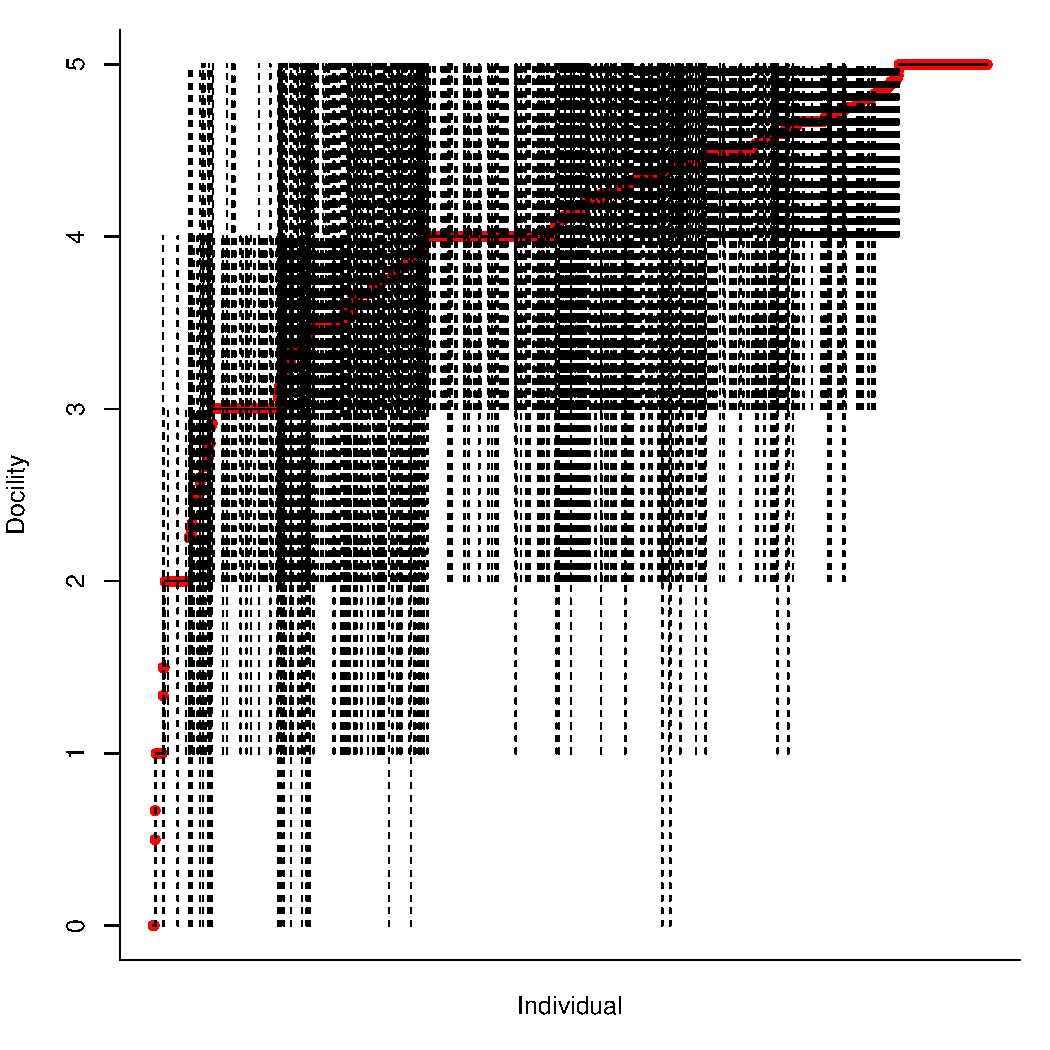
\includegraphics[width=14cm]{Figind.pdf}
		\end{center}
	\end{figure}
	
	\newpage
	\begin{figure}[H]
		\caption{Posterior mode and 95\% credible intervals for four different models of docility of Yellow-bellied marmots at RMBL. 
			Analysis used 11,389 observations from 1,576 individuals over 13 years. 
			Grey shaded area illustrates an invalid region of the parameter space. 
			Residual variance ($\sigma_e^2$) for models 3 and 4 were estimated based on Appendix \ref{ESM:equations}. 
			Juvenile was considered as references in both mean and variance part of the model.
			3.7 was subtracted from the estimates of the intercept to facilitate plotting.
		}
		\label{Fig:noyr}
		\begin{center}
			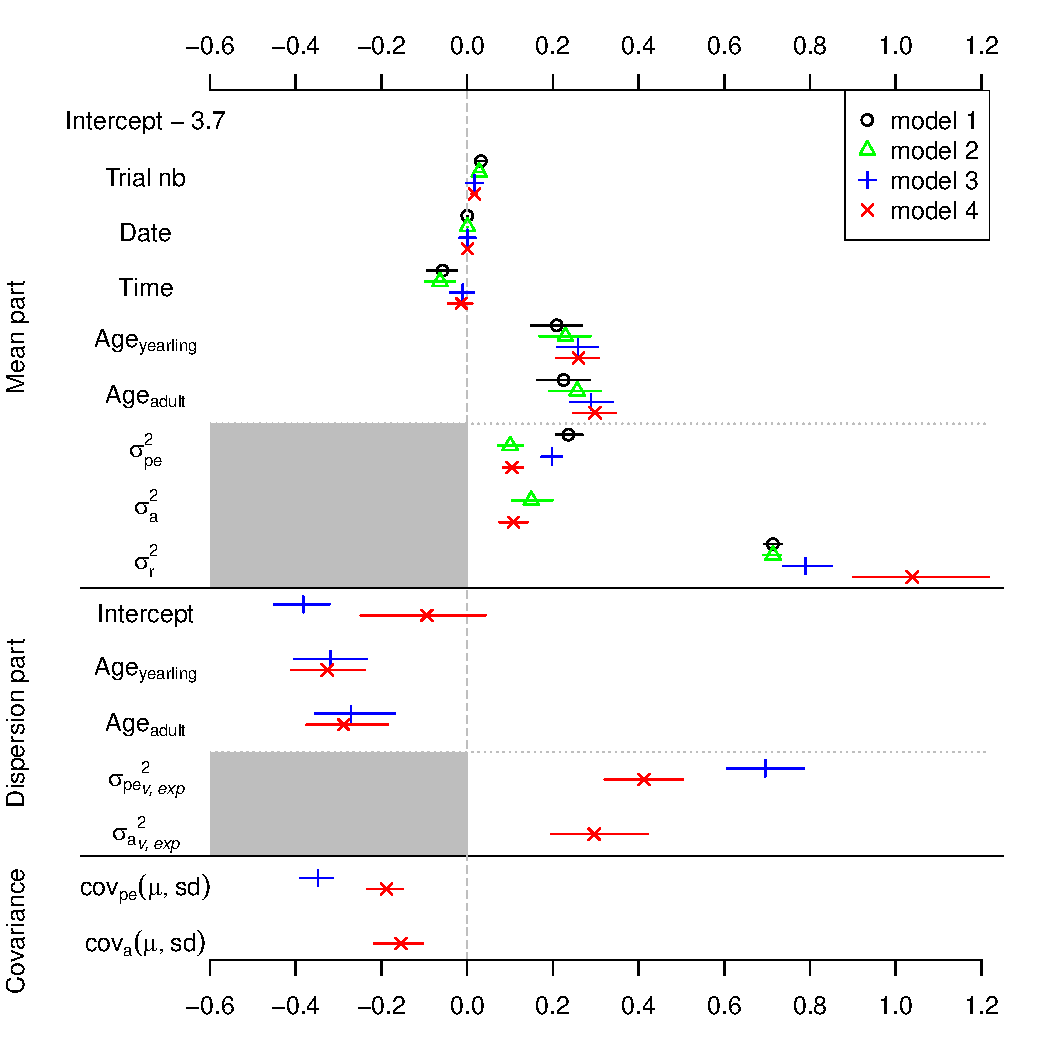
\includegraphics[width=14cm]{Fig1noyear.pdf}
		\end{center}
	\end{figure}
	
	
	\newpage
	\subsection{Annotated code to fit model 4 in OpenBugs}\label{ESM:bugscode}
	The code is also available in the file model4\_bugs.r
	\lstinputlisting{model4_bugs.r}
	
	\newpage
	\subsection{Calculation of variance ratios for double hierarchical models.}\label{ESM:equations}
	
	The aim here is to show the extension of the method presented in \citep{Mulder2007} to multiple random effects and how other parameters can be calculated.
	\cite{Felleki2012} and \cite{Sae-lim2015} showed derivations to estimate the heritability and permanent environment effect for within-individual variance.
	Using their approach, we reported their equations to estimate similar parameter when 3 random effects are included in the dispersion part of the model.
	First, it should be noted that the double hierarchical animal model (equation~\ref{Eq:dham}) could also be written in an additive way allowing an easier understanding of the estimations of the variance components and their ratios \citep{Sancristobal-gaudy1998}.
	\begin{equation}\label{Eq:dhamscg}
		\begin{aligned}
			\boldsymbol{Y} = &\boldsymbol{X_m b_m} + \boldsymbol{M yr_m} + \boldsymbol{Z pe_m} + \boldsymbol{Z a_m}\\
			&+ \chi \exp[1/2(\boldsymbol{X_v b_v} + \boldsymbol{M yr_v} + \boldsymbol{Z pe_v} + \boldsymbol{Z a_v})]
		\end{aligned}
	\end{equation}
	where $\chi \sim N(0,1)$ is a normal deviate.
	
	The residual variance $\sigma_e^2$ is calculated as:
	\begin{equation}
		\sigma_e^2 = \sigma_{e,exp}^2 \exp \left( \frac{\sigma_{yr_{v,exp}}^2}{2} \right) \exp \left( \frac{\sigma_{pe_{v,exp}}^2}{2} \right) \exp \left( \frac{\sigma_{a_{v,exp}}^2}{2} \right)
	\end{equation}
	
	In our analysis, the dispersion part of the model included three age categories as fixed effect.
	Thus assuming that the three age categories are equally represented in the sample, we can estimate $\sigma_{e,exp}^2$ as $\left( b_{v_0} + \frac{b_{v_1}}{3}+ \frac{b_{v_2}}{3} \right)$.
	The sum of the genetic, permanent environmental and year variance for the additive model can be calculated as:
	\begin{equation}
		\begin{aligned}
			\sigma_{a_v}^2 + \sigma_{pe_v}^2 + \sigma_{yr_v}^2 = \sigma_{e,exp}^4 \exp (2\sigma_{a_v,exp}^2)\exp (2\sigma_{pe_v,exp}^2)\exp (2\sigma_{yr_v,exp}^2) - \sigma_e^4
		\end{aligned}
	\end{equation}
	
	The product of equation (2) is a combination of $\sigma_{a_v}^2$, $\sigma_{pe_v}^2$ and $\sigma_{yr_v}^2$.
	Under the assumption that the ratio of $\frac{\sigma_{a_v}^2}{\sigma_{a_v}^2 + \sigma_{pe_v}^2 + \sigma_{yr_v}^2}$ is equal on both the additive and exponential scales, $\sigma_{a_v}^2$ is calculated as:
	\begin{equation}
		\sigma_{a_v}^2 = (\sigma_{yr_v}^2 + \sigma_{pe_v}^2 + \sigma_{a_v}^2 ) \frac{\sigma_{a_{v,exp}}^2}{\sigma_{yr_{v,exp}}^2 + \sigma_{pe_{v,exp}}^2 + \sigma_{a_{v,exp}}^2}
	\end{equation}
	
	Similarly, $\sigma_{pe_v}^2$ and $\sigma_{yr_v}^2$ are estimated as:
	\begin{align}
		\sigma_{pe_v}^2 &= (\sigma_{yr_v}^2 + \sigma_{pe_v}^2 + \sigma_{a_v}^2 ) \frac{\sigma_{pe_{v,exp}}^2}{\sigma_{yr_{v,exp}}^2 + \sigma_{pe_{v,exp}}^2 + \sigma_{a_{v,exp}}^2}\\
		\sigma_{yr_v}^2 &= (\sigma_{yr_v}^2 + \sigma_{pe_v}^2 + \sigma_{yr_v}^2 ) \frac{\sigma_{yr_{v,exp}}^2}{\sigma_{a_{v,exp}}^2 + \sigma_{pe_{v,exp}}^2 + \sigma_{yr_{v,exp}}^2}
	\end{align}
	
	Variance ratios including heritability ($h^2$) and repeatability ($r^2$) are important parameters in ecology and evolution \citep{Lynch1998, Roff2002}. 
	To ease comparison with other traits and standardize results of heterogeneity of within-individual variance, \cite{Mulder2007} defined a measure of heritability ($h_v^2$) for the within-individual variance in a trait.
	They proposed that ($h_v^2$) equals the genetic variance in within-individual variance as a proportion of the variance of the square of the trait, $P^2$.
	Thus, the heritability for within-individual variance ($h_v^2$) can be calculated as:
	\begin{equation}
		h_v^2 = \frac{\sigma_{a_v}^2}{2\sigma_P^4+3(\sigma_{yr_v}^2+ \sigma_{pe_v}^2 + \sigma_{a_v}^2)}
	\end{equation}
	
	Similarly, permanent environment ($pe^2$) and year ($year^2$) can be calculated as:
	\begin{align}
		pe_v^2 &= \frac{\sigma_{pe_v}^2}{2\sigma_P^4+3(\sigma_{yr_v}^2+ \sigma_{pe_v}^2 + \sigma_{a_v}^2)}\\
		year_v^2 &= \frac{\sigma_{yr_v}^2}{2\sigma_P^4+3(\sigma_{yr_v}^2+ \sigma_{pe_v}^2 + \sigma_{a_v}^2)}
	\end{align}
	
	For these equations, it is assumed that genetic ($r_a$) and permanent environmental ($r_{pe}$) correlations between mean and within individual variance are 0, otherwise the denominator would be slightly higher with the exponential model \citep{Mulder2007}.
	Even if the effect of this simplifying assumption seems to be weak \citep{Mulder2007, Sae-lim2015}, $h_v^2$ should be used only as a first approximation in standard prediction evolutionary model when $r_a=0$ .

	
\end{document}




